\documentclass[11pt]{article}
\usepackage[margin=1in]{geometry}
\usepackage[T1]{fontenc}
\usepackage{lmodern}
\usepackage{amsmath,amssymb,booktabs,graphicx,caption,xcolor,enumitem}
\usepackage[numbers,square,sort&compress]{natbib}
\usepackage[hidelinks]{hyperref}
\usepackage{microtype}
\graphicspath{{figures/}}
\captionsetup{font=small,labelfont=bf}
\setlist{itemsep=1pt,topsep=3pt}
\newcommand{\E}{\mathbb{E}}
\newcommand{\Var}{\operatorname{Var}}
\newcommand{\logit}{\operatorname{logit}}
\definecolor{boxbg}{HTML}{EEF4FC}
\newcommand{\keybox}[1]{\par\smallskip\noindent\colorbox{boxbg}{\parbox{\dimexpr\textwidth-2\fboxsep}{#1}}\par\smallskip}

\title{Does Bayesian Parameter Uncertainty Improve GARCH Volatility Forecasts and Volatility-Targeted Investing?\\[4pt]
\large Course project --- Erd\H{o}s Institute Quantitative Methods in Finance, Fall 2026}
\author{Kang Yu}
\date{November 2026}

\begin{document}
\maketitle

\begin{abstract}
\noindent
We ask whether accounting for Bayesian parameter uncertainty in a Gaussian GARCH(1,1) model improves (H1) one-day-ahead
conditional variance forecasts, (H2) predictive distributions of daily returns, and (H3) volatility-targeted
investment between an exchange-traded fund (ETF) and cash. Four ETFs (SPY, QQQ, TLT, GLD) are forecast out of sample
with rolling 500- and 1000-day windows, refitted every 63 trading days. Results are reported for a primary
evaluation period (2017--2022) and for a previously inspected period (2023--2026). \textbf{H1:} posterior-integrated
variance forecasts lower the QLIKE loss by about 0.005 (Diebold--Mariano $p=0.10$ and $0.08$), which is not
statistically reliable. \textbf{H2:} the posterior predictive mixture improves the log predictive score by a small
but significant 0.002--0.005 nats per day; a classical Laplace approximation captures 43--89\% of this gain. A
Student-$t$ GARCH model estimated by maximum likelihood improves the score about five to six times as much in
2017--2022 (3.6 to 7.5 times across all period--window cells), because parameter uncertainty adds far too little
tail mass to explain the observed fat tails. \textbf{H3:} a conservative rule based on the posterior 90th percentile
of variance holds 3.6 percentage points less risky exposure than the MLE rule and has shallower drawdowns in all
eight asset--window configurations. Against an exposure-matched MLE control, calibrated only on past data, the
drawdown advantage disappears, and every 95\% block-bootstrap interval for the Sharpe-ratio difference of the
equal-weight four-ETF sleeve contains zero. Two findings
stand out: innovation-distribution specification matters more for density forecasts than parameter uncertainty in
the Gaussian model, and lower drawdowns that come with lower exposure are not evidence of better risk timing.
\end{abstract}

\tableofcontents
\bigskip

% =====================================================================================================
\section{Research question and motivation}\label{sec:intro}
\paragraph{Research question.} \emph{Does accounting for Bayesian parameter uncertainty improve conditional variance
forecasts, predictive return distributions, and investment performance?}

\paragraph{Motivation.}
\begin{itemize}
\item \textbf{Volatility clustering.} Large price moves are followed by large moves. Daily returns are almost
uncorrelated, but squared returns are strongly autocorrelated (lag-1 autocorrelation 0.42 for SPY over 2013--2026), so
volatility is forecastable. GARCH(1,1) \cite{bollerslev1986}, which generalises the ARCH model of \citet{engle1982}, is the benchmark model for this and is notoriously hard
to beat out of sample \cite{hansenlunde2005}.
\item \textbf{Parameter uncertainty.} The three GARCH parameters are estimated from a few years of noisy daily data,
and persistence often lies close to the stationarity boundary. Standard practice nevertheless plugs in the point
estimate as if it were exact. A Bayesian treatment \cite{ardia2008} instead averages forecasts over the posterior.
\item \textbf{Heavy tails.} Daily returns, even after standardising by a GARCH forecast, have far more extreme days
than a normal distribution allows.
\item \textbf{A variance is not a distribution.} Two forecasts can agree on the variance yet assign very different
probabilities to a crash. Evaluating the variance and evaluating the whole predictive distribution are different questions.
\item \textbf{A statistical gain is not an economic gain.} A forecast can be more accurate without producing better
investment decisions, and a strategy can look safer simply because it holds less risk.
\end{itemize}

\paragraph{Hypotheses.}
\begin{description}
\item[H1 (conditional variance).] Bayesian parameter integration improves one-step-ahead conditional variance point
forecasts relative to Gaussian GARCH maximum likelihood (MLE).
\item[H2 (predictive distribution).] Bayesian parameter integration improves the full predictive distribution of
daily returns.
\item[H3 (investment performance).] Using Bayesian posterior uncertainty in volatility-targeted allocation produces
better investment outcomes, beyond merely reducing risky exposure.
\end{description}
\noindent Each hypothesis is treated in turn (Sections~\ref{sec:h1}--\ref{sec:h3control}) with the same structure:
the question, how it is investigated, the evaluation metric and why it is appropriate, the numerical results, and
the conclusion. Two results receive particular emphasis: the comparison with Student-$t$ GARCH under H2, and the
exposure-matched control experiment under H3. The empirical design, models and data splits were fixed before the
2017--2022 period was evaluated.

% =====================================================================================================
\section{Statistical methodology}\label{sec:method}
\subsection{Gaussian GARCH(1,1) and maximum likelihood}
Let $r_t$ be the daily log return of an ETF's adjusted closing price and $\mathcal F_{t-1}$ the information up to
day $t-1$. The model is
\begin{equation}\label{eq:garch}
r_t=\sqrt{h_t}\,z_t,\quad z_t\overset{iid}{\sim}N(0,1),\qquad h_t=\omega+\alpha r_{t-1}^2+\beta h_{t-1}.
\end{equation}
$h_t=\Var(r_t\mid\mathcal F_{t-1})$ is the \emph{conditional variance}: it is known one day in advance, and a large
shock raises tomorrow's variance (volatility clustering). Positivity requires $\omega>0$ and $\alpha,\beta\ge0$;
covariance stationarity requires the \emph{persistence} $p=\alpha+\beta<1$. Then $V=\omega/(1-p)$ is the long-run
(unconditional) variance and forecasts revert to it geometrically,
$\E[h_{t+k}\mid\mathcal F_t]-V=p^{k-1}(h_{t+1}-V)$, with half-life $\log 0.5/\log p$ days.

\paragraph{Likelihood and estimation.} Conditional on $h_1$, the Gaussian log-likelihood is
\begin{equation}\label{eq:loglik}
\ell(\theta)=-\tfrac12\sum_t\bigl[\log 2\pi+\log h_t(\theta)+r_t^2/h_t(\theta)\bigr],
\end{equation}
computed by running the recursion~\eqref{eq:garch} from $h_1=V$. The implementation (\texttt{bgarch.garch}) optimises
in unconstrained coordinates $u=(\log V,\logit p,\logit q)$ with $q=\alpha/p$, so that $\omega=V(1-p)$, $\alpha=pq$,
$\beta=p(1-q)$ and every point satisfies the constraints. These coordinates are also far better conditioned than
$(\omega,\alpha,\beta)$. The likelihood is maximised by multi-start L-BFGS-B with box bounds $\logit p\in[-7,7]$ and a
Powell fallback; the bound caps persistence at $p\le0.99909$. On equity and bond data the likelihood often keeps
rising toward $p=1$ and the optimiser stops \emph{on the bound}: this happens in 30 of the 320 refits
(Appendix~\ref{app:robust}).

\subsection{Bayesian Gaussian GARCH}
\paragraph{Prior and posterior.} The prior is independent Gaussian on the unconstrained coordinates,
$\log V\sim N(\log10^{-4},1.5^2)$, $\logit p\sim N(\logit0.8,1.5^2)$, $\logit q\sim N(\logit0.1,1.5^2)$. It is a
density in $u$, so no Jacobian is required, and it shrinks near-integrated estimates away from $p=1$. The posterior
is $\pi(u\mid D)\propto e^{\ell(u)}\pi(u)$, where $D$ is the estimation window.

\paragraph{Sampling and convergence.} The posterior is sampled by random-walk Metropolis with four over-dispersed
chains. The proposal covariance and scale are adapted during 2{,}500 warm-up iterations, targeting 23.4\% acceptance
\cite{roberts1997,haario2001}, and adaptation is frozen for the 4{,}000 retained draws per chain. A fit passes only if
the rank-normalised $\hat R<1.01$ and bulk and tail effective sample sizes are $\ge400$ for every parameter
\cite{vehtari2021}. Table~\ref{tab:fits} summarises convergence over the 320 refits. The sampler agrees with an
independent importance sampler to within 0.3\% for posterior means and quantiles of next-day variance.

\paragraph{From posterior draws to forecasts.} Each retained draw $u^{(m)}$, $m=1,\dots,M$ ($M=300$ draws sampled at random, without replacement, from the 16{,}000 retained draws of each refit),
runs its own variance recursion and gives its own forecast $h_t^{(m)}=h_t(u^{(m)})$. The distribution of
$\{h_t^{(m)}\}$ describes uncertainty about the \emph{forecast}, not about the return. Three summaries are used,
one per hypothesis:
\begin{align}
\text{H1:}\quad&\bar h_t=\frac1M\sum_m h_t^{(m)}\approx\E_{\theta\mid D}[h_t(\theta)] &&\text{(posterior-integrated variance)}\\
\text{H2:}\quad&p_{\text{Bayes}}(r)=\frac1M\sum_m N\bigl(r;0,h_t^{(m)}\bigr) &&\text{(posterior predictive mixture)}\label{eq:mixture}\\
\text{H3:}\quad&q_{0.9,t}=\text{90th percentile of }\{h_t^{(m)}\} &&\text{(cautious ``upper-90'' variance)}
\end{align}
The MLE forecast instead evaluates the model at a single point, $h_t(\hat u)$, and uses the single density
$N(r;0,h_t(\hat u))$. A third forecast, the \emph{posterior-mean plug-in} $h_t(\bar u)$ with $\bar u$ built from the
posterior means of $(V,p,q)$, isolates the effect of prior shrinkage from that of integration.

\paragraph{Averaging densities, not log densities.} The predictive density~\eqref{eq:mixture} averages the component
densities and only then takes the logarithm when it is scored. By Jensen's inequality (concavity of the logarithm),
$\log\frac1M\sum_m p_m(r)\ge\frac1M\sum_m\log p_m(r)$ for every realised $r$: the score of the mixture is never below
the average score of its components, with equality only when all components agree at $r$. The right-hand side is
\emph{not} the score of any predictive density: $\exp\{\frac1M\sum_m\log p_m(r)\}$ is the geometric mean of the
component densities, which integrates to less than one unless all components coincide. Averaging log densities is
therefore not a valid substitute for the mixture. The implementation (\texttt{bgarch.forecast.mixture\_logpdf}) uses
a log-sum-exp.

\paragraph{Monte Carlo variability.} MCMC outputs are random, and starting points are generated through a
linear-algebra routine whose output varies across platforms. Bayesian columns therefore reproduce to Monte Carlo
precision rather than bit-for-bit across machines (Appendix~\ref{app:robust}).

\subsection{Student-\texorpdfstring{$t$}{t} GARCH, estimated by maximum likelihood}
Student-$t$ GARCH \cite{bollerslev1987} keeps the variance recursion~\eqref{eq:garch} but replaces the normal
innovation by a standardised Student-$t$ variable, $z_t=\sqrt{(\nu-2)/\nu}\,T_\nu$ with $\nu>2$, so that
$\Var(z_t)=1$ and $h_t$ is still the conditional variance. The conditional log density is
\begin{equation}\label{eq:tdens}
\log f(r_t\mid h_t)=\log\Gamma\!\bigl(\tfrac{\nu+1}2\bigr)-\log\Gamma\!\bigl(\tfrac\nu2\bigr)-\tfrac12\log\bigl(\pi(\nu-2)h_t\bigr)
-\tfrac{\nu+1}{2}\log\Bigl(1+\frac{r_t^2}{(\nu-2)h_t}\Bigr).
\end{equation}
The degrees-of-freedom parameter $\nu$ controls the tails: the excess kurtosis of $z_t$ is $6/(\nu-4)$ for $\nu>4$
and infinite for $\nu\le4$, while $\nu\to\infty$ recovers the normal. Compared with the Gaussian
likelihood~\eqref{eq:loglik}, a large standardised return is penalised \emph{logarithmically} rather than
quadratically, so a single extreme day does not force the variance up as strongly, and the predictive density
assigns non-negligible probability to four- and five-sigma days. The model is \emph{fully implemented and estimated
in this project} (\texttt{bgarch.student\_t}): the four parameters $(u,\nu)$ are found by multi-start L-BFGS-B with
the same box bounds on $u$ as the Gaussian MLE and $\nu\in(2.05,202)$, at every one of the 320 refits. The fitted
$\nu$ has a median of 7.2 (SPY 6.1, QQQ 6.8, GLD 5.9, TLT 17.7); 7 refits (6 TLT, 1 QQQ) reach the upper bound, i.e.
an essentially Gaussian fit.

\keybox{\small\textbf{Two mechanisms for heavier predictive tails.} \emph{Bayesian Gaussian GARCH} adds predictive
uncertainty by mixing Gaussians whose variances differ across parameter draws; the extra tail mass depends on how
dispersed the posterior forecasts $h_t^{(m)}$ are. \emph{Student-$t$ GARCH} builds heavy-tailed innovations directly
into the conditional return model, independently of parameter uncertainty. The H2 results (Section~\ref{sec:h2})
are interpreted through this distinction.}

\subsection{Other comparators}
\begin{itemize}
\item \textbf{Laplace approximation} (classical estimation uncertainty): draws from $N(\hat u,\hat{\mathcal I}^{-1})$,
where $\hat{\mathcal I}$ is the observed information at the MLE, turned into a variance mixture and a 90th
percentile exactly like the posterior draws. It asks how much of any Bayesian gain comes from acknowledging
estimation uncertainty at all, without MCMC.
\item \textbf{EWMA} with $\lambda=0.94$ \cite{riskmetrics1996}, the industry baseline.
\item \textbf{MAP} and the posterior-mean plug-in, which separate shrinkage from integration.
\end{itemize}

% =====================================================================================================
\section{Data and rolling experimental design}\label{sec:design}
\paragraph{Data.} Daily dividend- and split-adjusted closes of SPY and QQQ (US equities), TLT (long Treasury bonds) and
GLD (gold), 2013-01-02 to 2026-11-04, from Yahoo Finance; daily log returns start on 2013-01-03. The cash rate is
the effective federal funds rate (FRED series DFF). Provenance is in Appendix~\ref{app:data}.

\paragraph{Rolling design.} Figure~\ref{fig:design} shows the forecasting procedure. Five objects must be kept apart:
\begin{enumerate}
\item the \textbf{complete return history} from 2013, from which estimation windows are drawn;
\item the \textbf{moving estimation window}: the last $W=500$ or $1{,}000$ returns \emph{before} a refit date;
\item the \textbf{evaluation dates}: every trading day of the evaluation period receives a one-step-ahead forecast;
\item the \textbf{refitting schedule}: parameters (MLE, posterior draws, Laplace, Student-$t$) are re-estimated every
63 trading days and then frozen;
\item the \textbf{daily variance updates}: between refits, every model's recursion is updated each day with the newly
observed return, so the forecast for day $d$ always uses $r_{d-1}$.
\end{enumerate}
\noindent Each day the procedure is: returns up to $d-1$ are known $\rightarrow$ the current parameters (from the most
recent refit, whose window ended before the refit date) give $h_d$ $\rightarrow$ the forecast for day $d$ is made
$\rightarrow$ $r_d$ is observed and the forecast scored $\rightarrow$ move to $d+1$. Saved forecast files are checked
for this ordering: every row's fit window ends strictly before the row date. Over 4 ETFs, 2 windows and 2 periods
this gives 320 refits.

\begin{figure}[t]\centering
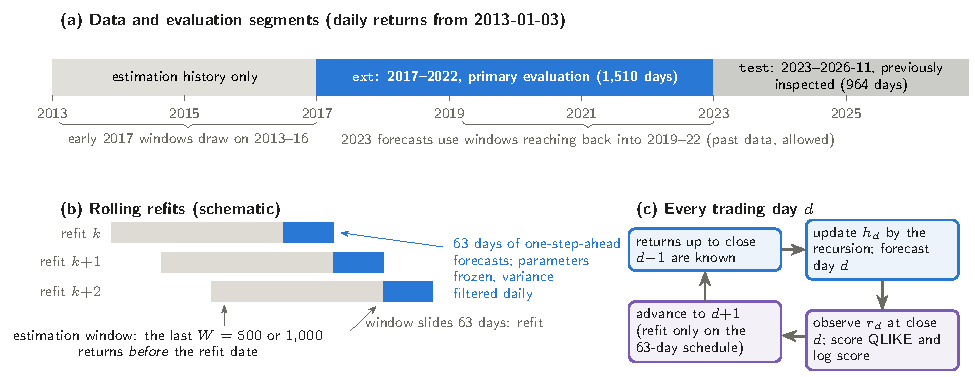
\includegraphics[width=\textwidth]{rolling_design.pdf}
\caption{Rolling out-of-sample design. (a) Evaluation segments. (b) Each refit estimates every model on the last $W$
returns and then forecasts the next 63 trading days with the parameters frozen. (c) The daily loop: the variance is
updated every day, while parameters change only at refits.}\label{fig:design}
\end{figure}

\paragraph{Evaluation segments.} The label \texttt{ext} denotes 2017-01-03 to 2022-12-30 (1{,}510 days per ETF), the
\textbf{primary evaluation}. It is independent of earlier research-development \emph{inspection}: the models,
metrics and decision rules were frozen before any 2017--2022 result was examined. This does not mean that its
returns or estimation windows are statistically independent of anything else. The label \texttt{test} denotes
2023-01-03 to 2026-11-04 (964 days), a period studied repeatedly in earlier project milestones and therefore reported
only as a reproduction. Both segments consist of chronological out-of-sample forecasts; neither is a ``training
set''. Earlier returns legitimately enter the estimation windows of later forecasts: for example, the 1000-day windows
used in 2023 reach back into 2019--2022, and the first 2017 windows draw on 2013--2016.

\begin{table}[h]\centering\small
\begin{tabular}{lrrrrrr}\toprule
Period & refits & failed strict diag. & max $\hat R$ & min tail ESS & MLE on $p$-bound & median $\hat\nu$ ($t$-GARCH)\\\midrule
2017--22 & 192 & 2 & 1.019 & 254 & 15 & 5.6 \\
2023--26 & 128 & 2 & 1.010 & 502 & 15 & 11.9 \\
\bottomrule\end{tabular}

\caption{Fit diagnostics over the 320 refits (moderate prior, 4 ETFs $\times$ 2 windows, quarterly refits). A
``failure'' means the strict convergence rule was missed. All four failures are marginal, and excluding their
forecast days leaves the forecast comparisons unchanged.}\label{tab:fits}
\end{table}

% =====================================================================================================
\section{H1: conditional variance forecasting}\label{sec:h1}
\paragraph{Question.} Does accounting for parameter uncertainty improve conditional variance point forecasts? The
competing forecasts for day $t$, both formed from $r_{<t}$ only, are
\[
\hat h_t^{\text{MLE}}=h_t(\hat\theta),\qquad \hat h_t^{\text{Bayes}}=\E_{\theta\mid D_{t-1}}[h_t(\theta)]\approx\bar h_t.
\]

\paragraph{The evaluation problem.} The true conditional variance $h_t$ is never observed. The squared return is an
unbiased proxy, $\E[r_t^2\mid\mathcal F_{t-1}]=h_t$, but a very noisy one: under normality $r_t^2/h_t\sim\chi^2_1$,
whose standard deviation is $\sqrt2$ times its mean. A loss function must therefore rank forecasts correctly
\emph{on average} even though each day's target is mostly noise.

\paragraph{Metric: QLIKE.}
\begin{equation}\label{eq:qlike}
\text{QLIKE}_t(\hat h)=\log\hat h_t+\frac{r_t^2}{\hat h_t}\qquad\text{(lower is better).}
\end{equation}
\textit{Derivation.} Let $h^*=\E[r_t^2\mid\mathcal F_{t-1}]$ be the true conditional variance. Taking conditional
expectations, $\E[\text{QLIKE}_t(\hat h)\mid\mathcal F_{t-1}]=\log\hat h+h^*/\hat h$. Its derivative in $\hat h$ is
$1/\hat h-h^*/\hat h^2$, which vanishes only at $\hat h=h^*$, and the second derivative there is $1/h^{*2}>0$.
Equivalently, the expected excess loss of any forecast is
\[
\E[\text{QLIKE}_t(\hat h)-\text{QLIKE}_t(h^*)\mid\mathcal F_{t-1}]=x-1-\log x\ \ge0,\qquad x=h^*/\hat h,
\]
with equality only at $x=1$. Three consequences follow.
\begin{enumerate}
\item Expected QLIKE is minimised by the true conditional variance, so the ranking of two forecasts by \emph{expected}
QLIKE is the same whether they are scored against the noisy proxy or the latent variance \cite{patton2011}. On any
single day, and in a finite sample, the proxy noise remains, which is why average differences are tested statistically.
\item The argument uses only $\E[r_t^2\mid\mathcal F_{t-1}]=h^*<\infty$ (zero conditional mean and a finite conditional
second moment); it does \emph{not} require Gaussian returns, which
matters because the returns are heavy-tailed (Section~\ref{sec:h2}).
\item Up to scaling and an additive constant, QLIKE is the Gaussian negative log-likelihood:
$-\log N(r_t;0,\hat h_t)=\tfrac12[\log2\pi+\text{QLIKE}_t]$.
\end{enumerate}
QLIKE penalises under-prediction more than over-prediction ($x-1-\log x$ grows linearly as $x\to\infty$ but only
logarithmically as $x\to0$), which is appropriate for risk forecasting.

\paragraph{Statistical comparison.} For two methods A and B, the daily loss differences
$d_t=\text{QLIKE}_t(A)-\text{QLIKE}_t(B)$ are averaged across the four ETFs on each day (``pooled''), and their mean is
tested with a Diebold--Mariano test \cite{diebold1995} using Newey--West standard errors \cite{neweywest1987}, which
allow for serial correlation and heteroskedasticity in $d_t$.

\paragraph{Results.} Table~\ref{tab:qlike} and Figure~\ref{fig:qlike} report the contrasts. Average QLIKE is about
$-8.3$ in 2017--22 (for example, $-8.317$ for MLE and $-8.322$ for the integrated forecast, averaged over ETFs with the
500-day window), so the differences are a few thousandths.
\begin{itemize}
\item \textbf{Bayes integrated $-$ MLE:} $-5.3\times10^{-3}$ and $-5.6\times10^{-3}$ in 2017--22 ($p=0.105$, $0.076$);
$-3.3\times10^{-3}$ and $-0.8\times10^{-3}$ in 2023--26 ($p=0.21$, $0.48$). The sign favours the Bayesian forecast in
every cell, but no difference is significant at 5\%.
\item \textbf{Decomposition:} in 2017--22 most of the small difference comes from shrinkage (posterior-mean plug-in $-$ MLE);
integration on its own changes QLIKE by about $10^{-3}$, with either sign.
\item \textbf{Window length:} the 1000-day window gives slightly larger point differences in 2017--22 and smaller ones
in 2023--26; none is significant.
\item For reference, Student-$t$ GARCH also gives a lower QLIKE than MLE in 2017--22 ($-6.0$ and $-8.9\times10^{-3}$,
the latter with $p=0.016$), of a similar size to the Bayesian contrast; EWMA is worse than MLE.
\end{itemize}

\begin{table}[h]\centering\footnotesize
\resizebox{\textwidth}{!}{\begin{tabular}{lrrrr}\toprule
 & \multicolumn{2}{c}{2017--22 (primary)} & \multicolumn{2}{c}{2023--26 (previously inspected)}\\\cmidrule(lr){2-3}\cmidrule(lr){4-5}
Contrast ($\times10^{-3}$, DM $p$-value) & $W{=}500$ & $W{=}1000$ & $W{=}500$ & $W{=}1000$\\\midrule
Bayes integrated $-$ MLE & -5.34 (.105) & -5.58 (.076) & -3.31 (.206) & -0.85 (.484) \\
posterior-mean plug-in $-$ MLE (shrinkage only) & -4.30 (.280) & -6.39 (.100) & -1.75 (.652) & -0.21 (.912) \\
integrated $-$ mean plug-in (integration only) & -1.04 (.448) & +0.81 (.459) & -1.56 (.390) & -0.64 (.540) \\
Student-$t$ $-$ MLE & -5.98 (.116) & -8.92 (.016) & +0.12 (.961) & -0.13 (.928) \\
EWMA $-$ MLE & +14.08 (.340) & +16.37 (.303) & +6.69 (.524) & +11.19 (.229) \\
\bottomrule\end{tabular}
}
\caption{H1. Pooled four-ETF Diebold--Mariano contrasts of QLIKE. Entries are mean daily differences $\times10^{-3}$
(negative favours the first method) with Newey--West $p$-values.}\label{tab:qlike}
\end{table}

\begin{figure}[h]\centering
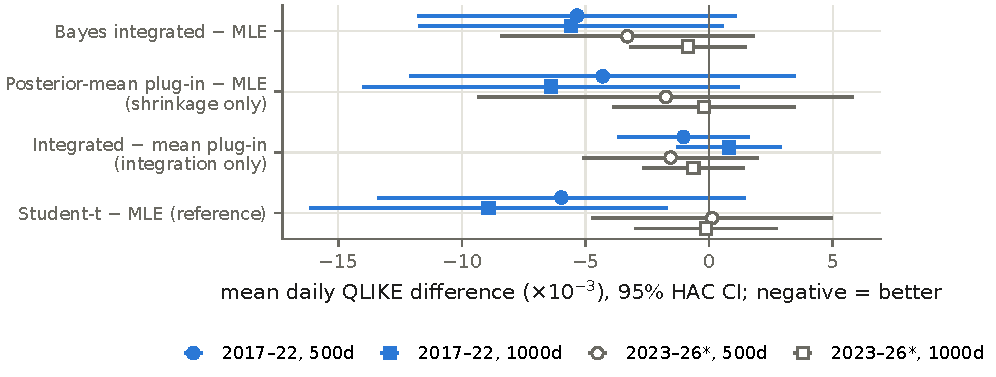
\includegraphics[width=.85\textwidth]{qlike_contrasts.pdf}
\caption{H1. Pooled QLIKE differences with 95\% Newey--West intervals. Filled: 2017--22 (primary); hollow:
2023--26 (previously inspected).}\label{fig:qlike}
\end{figure}

\paragraph{Conclusion for H1.} Posterior-integrated variance forecasts show small numerical improvements that are not
statistically reliable at the 5\% level in the primary evaluation. \textbf{H1 is not supported.} A non-significant
result is not proof that the forecasts are equivalent: the intervals in Figure~\ref{fig:qlike} are compatible both
with no effect and with a small gain.

% =====================================================================================================
\section{H2: predictive return distributions}\label{sec:h2}
\paragraph{Question and motivation.} Does accounting for parameter uncertainty improve the prediction of the
\emph{whole} distribution of daily returns? QLIKE cannot answer this: two models can have similar conditional variance
forecasts while assigning very different probabilities to extreme returns. On 5 February 2018, for example, SPY's
three predictive standard deviations were within 5\% of one another (17.8\%, 17.9\% and 17.0\% annualised for MLE,
Bayes and Student-$t$), yet the realised $-4.3\%$ return, $3.8$ MLE standard deviations, had a predictive density
about 8.6 times larger under Student-$t$ than under the Gaussian MLE (Figure~\ref{fig:dens}).

\paragraph{Metric: the log predictive score.} Each model states a predictive density before the return is observed,
and it is evaluated at the realised return:
\begin{equation}
S_t=\log p\bigl(r_t^{\text{obs}}\mid D_{t-1}\bigr)\qquad\text{(higher is better).}
\end{equation}
The log score is strictly proper \cite{gneiting2007}: its expectation is maximised only by the true predictive
distribution, so it rewards calibration and sharpness together and evaluates the full distribution, not just its
variance. For a single Gaussian predictive density, $-S_t=\tfrac12[\log2\pi+\text{QLIKE}_t]$, so comparing two Gaussian
plug-in forecasts by the log score is the same as comparing them by QLIKE. For a Gaussian mixture or a Student-$t$
density the two metrics differ: the log score also rewards the \emph{shape} of the distribution, in particular how
much mass it puts in the tails. Scores are compared with the same pooled Diebold--Mariano tests as in H1.

\paragraph{Three principal predictive densities.}
\begin{enumerate}
\item[A.] \textbf{Gaussian GARCH, MLE:} one Gaussian, $p(r)=N(r;0,h_t(\hat\theta))$.
\item[B.] \textbf{Bayesian Gaussian GARCH:} the posterior predictive mixture
\[
p_{\text{Bayes}}(r_t\mid D_{t-1})=\int N\bigl(r_t;0,h_t(\theta)\bigr)\,p(\theta\mid D_{t-1})\,d\theta
\approx\frac1M\sum_{m=1}^{M}N\bigl(r_t;0,h_t^{(m)}\bigr),
\]
a Monte Carlo approximation with $M=300$ posterior draws. Its width reflects both the innovation noise and the
uncertainty in $\theta$.
\item[C.] \textbf{Student-$t$ GARCH, MLE:} the density~\eqref{eq:tdens} with estimated $\hat\nu$, which addresses heavy
tails directly.
\end{enumerate}

\paragraph{Results.} Table~\ref{tab:ls} and Figure~\ref{fig:ls} report the contrasts and Table~\ref{tab:ratio} the
ratios.
\begin{itemize}
\item \textbf{Bayesian mixture $-$ MLE:} $+5.2$ and $+4.7\times10^{-3}$ nats per day in 2017--22 ($p=0.012$, $0.024$),
and $+5.2$ and $+2.3\times10^{-3}$ in 2023--26; significant in all four cells ($p\le0.024$). The mixture also beats the
posterior-mean plug-in density in every cell, so the gain comes from integration and not only from shrinkage.
\item \textbf{Classical uncertainty does much of the work:} the Laplace mixture achieves 43--89\% of the Bayesian gain
(more than half in three of the four cells). Much of the benefit comes from acknowledging estimation uncertainty
rather than from Bayesian inference as such.
\item \textbf{Student-$t$ $-$ MLE:} $+28.2$ and $+28.7\times10^{-3}$ in 2017--22, $+18.9$ and $+17.0\times10^{-3}$ in
2023--26. That is 5.4 and 6.1 times the Bayesian gain in 2017--22 and 3.6 to 7.5 times across all four cells; the
ratio is not constant across periods and windows. Student-$t$ also beats the Bayesian mixture directly in every cell
($p\le0.011$).
\end{itemize}

\begin{table}[h]\centering\footnotesize
\resizebox{\textwidth}{!}{\begin{tabular}{lrrrr}\toprule
 & \multicolumn{2}{c}{2017--22 (primary)} & \multicolumn{2}{c}{2023--26 (previously inspected)}\\\cmidrule(lr){2-3}\cmidrule(lr){4-5}
Contrast ($\times10^{-3}$, DM $p$-value) & $W{=}500$ & $W{=}1000$ & $W{=}500$ & $W{=}1000$\\\midrule
Bayes predictive mixture $-$ MLE & +5.18 (.012) & +4.69 (.024) & +5.19 (.015) & +2.26 (.024) \\
predictive mixture $-$ mean plug-in (integration only) & +3.03 (<.001) & +1.49 (.004) & +4.31 (.006) & +2.15 (<.001) \\
Laplace mixture $-$ MLE & +4.59 (<.001) & +2.03 (<.001) & +4.26 (.006) & +1.55 (.018) \\
Student-$t$ $-$ MLE & +28.22 (<.001) & +28.65 (<.001) & +18.87 (.005) & +16.99 (.002) \\
Student-$t$ $-$ Bayes predictive mixture & +23.03 (<.001) & +23.96 (<.001) & +13.69 (.011) & +14.73 (.002) \\
\bottomrule\end{tabular}
}
\caption{H2. Pooled four-ETF Diebold--Mariano contrasts of the log predictive score. Entries are mean daily
differences $\times10^{-3}$ nats (positive favours the first method) with Newey--West $p$-values.}\label{tab:ls}
\end{table}

\begin{figure}[h]\centering
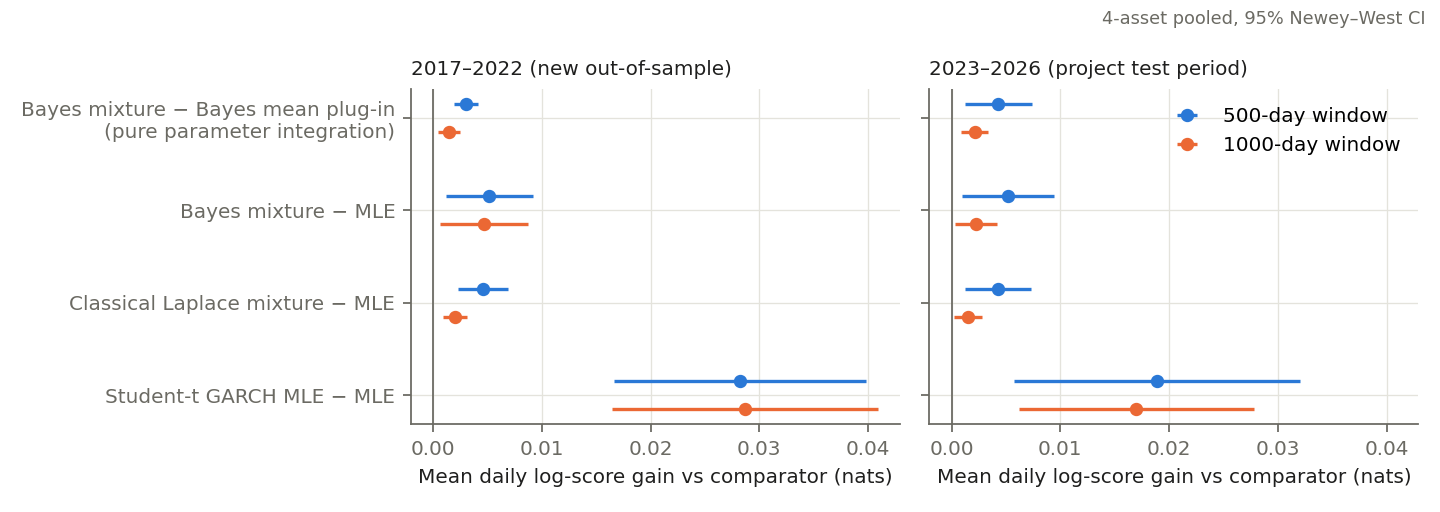
\includegraphics[width=.95\textwidth]{fig1_logscore_gains.png}
\caption{H2. Daily log-score gains with 95\% HAC intervals. Integrating over parameter uncertainty helps slightly;
modelling fat tails helps far more.}\label{fig:ls}
\end{figure}

\begin{table}[h]\centering\small
\begin{tabular}{lrrrr}\toprule
 & \multicolumn{2}{c}{2017--22 (primary)} & \multicolumn{2}{c}{2023--26 (previously inspected)}\\\cmidrule(lr){2-3}\cmidrule(lr){4-5}
Pooled log-score gain & $W{=}500$ & $W{=}1000$ & $W{=}500$ & $W{=}1000$\\\midrule
Bayes mixture $-$ MLE ($\times10^{-3}$) & +5.18 & +4.69 & +5.19 & +2.26 \\
Student-$t$ $-$ MLE ($\times10^{-3}$) & +28.22 & +28.65 & +18.87 & +16.99 \\
Student-$t$ gain $\div$ Bayesian gain & 5.44 & 6.11 & 3.64 & 7.52 \\
Laplace gain $\div$ Bayesian gain & 0.89 & 0.43 & 0.82 & 0.69 \\
\bottomrule\end{tabular}

\caption{Size of the Student-$t$ gain and of the Laplace gain relative to the Bayesian mixture gain, per period and
window.}\label{tab:ratio}
\end{table}

\subsection{Why does Student-\texorpdfstring{$t$}{t} GARCH perform so much better?}
The comparison between B and C is the central H2 finding, and it has a simple explanation.
\begin{enumerate}
\item \textbf{Gaussian GARCH already models time-varying variance.} Even with Gaussian innovations, a changing $h_t$
makes \emph{unconditional} returns heavy-tailed. The relevant question is whether the \emph{conditional} tails are right.
\item \textbf{Bayesian integration adds one more Gaussian scale mixture,} over the posterior spread of $h_t^{(m)}$.
\item \textbf{How much tail it adds is measurable.} If $r=\sqrt H\,z$ with $z\sim N(0,1)$ independent of the mixing
variance $H$, then $\E r^2=\E H$ and $\E r^4=3\E H^2$, so
\begin{equation}\label{eq:kurt}
\kappa_{\text{excess}}=\frac{\E r^4}{(\E r^2)^2}-3=3\,\frac{\Var(H)}{\E[H]^2}=3\,\mathrm{CV}^2 .
\end{equation}
This assumes zero mean and a mixing variance independent of the innovation, which holds for the predictive
mixture~\eqref{eq:mixture}, where $H$ is uniform over the posterior forecasts $h_t^{(m)}$.
\item \textbf{The posterior dispersion is limited.} The posterior coefficient of variation of next-day variance is
7--12\% on average; averaging $3\,\mathrm{CV}^2$ over days gives an implied excess kurtosis of only 0.015--0.046.
\item \textbf{The data need far more.} Returns standardised by the posterior-integrated forecast have excess kurtosis 0.4--2.9
(Figure~\ref{fig:k}). Parameter uncertainty can explain only a few per cent of the observed tail heaviness.
\item \textbf{Student-$t$ innovations supply it directly.} With a median $\hat\nu\approx7$, the conditional density
has excess kurtosis of order 2, the size actually observed. On 5 February 2018 the posterior CV was unusually high
(0.18, implied excess kurtosis 0.09), and the mixture's probability of a loss beyond four MLE standard deviations was
$6.8\times10^{-5}$, about twice the Gaussian's $3.2\times10^{-5}$ but forty times smaller than the Student-$t$
model's $2.7\times10^{-3}$ (Figure~\ref{fig:dens}).
\item \textbf{Residual diagnostics agree} (Appendix~\ref{app:adequacy}): Gaussian GARCH leaves standardised returns
with too many $|z|>3$ days, and 1\% value-at-risk is exceeded on about 2\% of days with or without posterior
integration, while Student-$t$ reduces this to 1.5\% in 2017--22 (Table~\ref{tab:var}).
\end{enumerate}

\begin{figure}[h]\centering
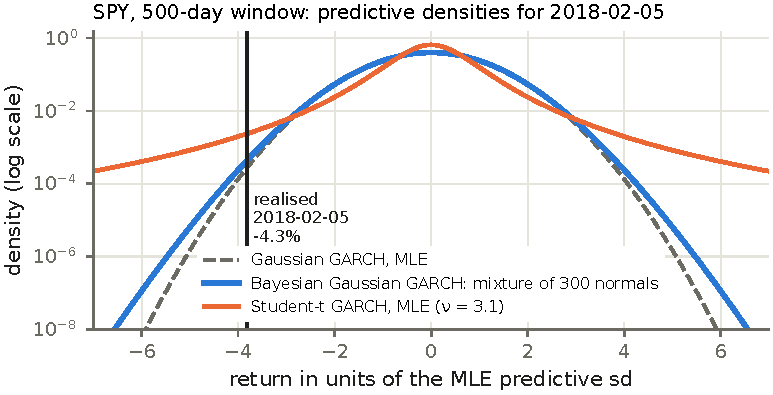
\includegraphics[width=.75\textwidth]{predictive_densities.pdf}
\caption{Predictive densities for one illustrative day (SPY, 500-day window, saved model estimates for 5 February
2018), on a log scale in units of the MLE predictive standard deviation. The Bayesian mixture is only slightly wider
in the tails than the Gaussian MLE; the Student-$t$ density ($\hat\nu=3.1$ on this refit) is far heavier-tailed. The
day was chosen to illustrate the tails, not as a typical day.}\label{fig:dens}
\end{figure}

\begin{figure}[h]\centering
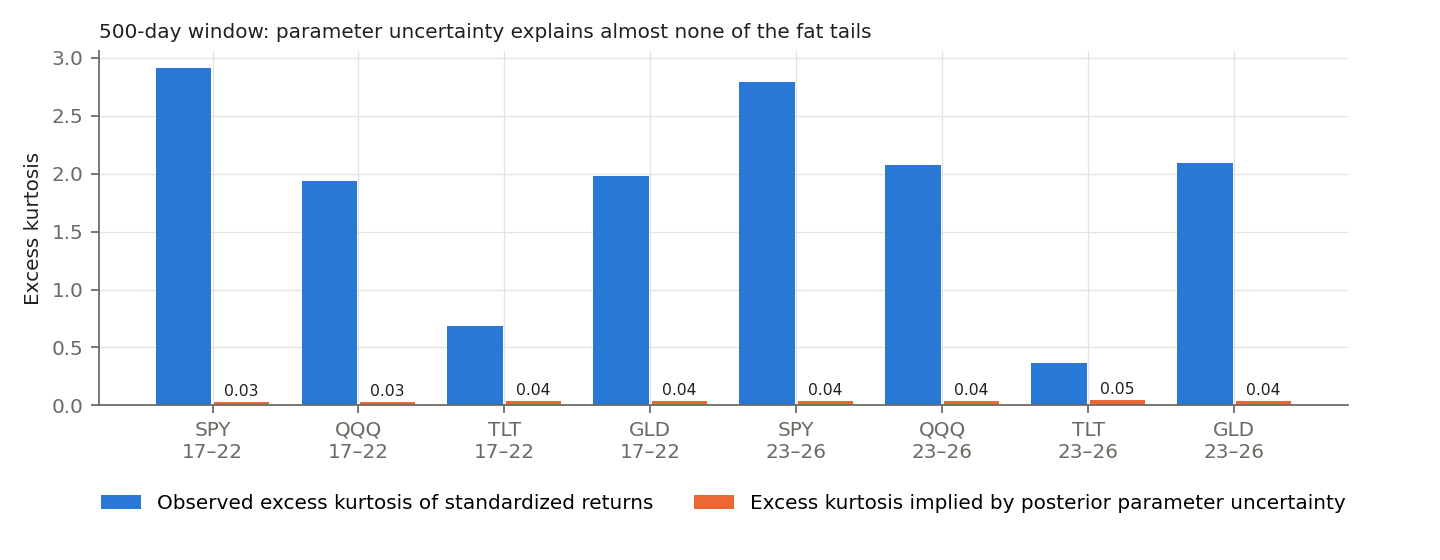
\includegraphics[width=.8\textwidth]{fig4_kurtosis.png}
\caption{Observed excess kurtosis of standardised returns versus the excess kurtosis implied by posterior parameter
uncertainty, $3\,\mathrm{CV}^2$ (500-day window).}\label{fig:k}
\end{figure}

\begin{table}[h]\centering\small
\begin{tabular}{lrrrr}\toprule
 & \multicolumn{2}{c}{2017--22} & \multicolumn{2}{c}{2023--26}\\\cmidrule(lr){2-3}\cmidrule(lr){4-5}
VaR violation rate \% (Kupiec rejections of 8) & 1\% & 5\% & 1\% & 5\%\\\midrule
Gaussian, MLE & 2.15 (8) & 5.89 (3) & 1.65 (4) & 5.10 (0) \\
Gaussian, posterior-mean plug-in & 2.02 (6) & 5.80 (2) & 1.54 (4) & 4.81 (1) \\
Bayesian predictive mixture & 2.06 (6) & 5.89 (3) & 1.58 (4) & 4.97 (0) \\
Laplace mixture & 2.09 (7) & 5.93 (3) & 1.57 (4) & 5.04 (0) \\
Student-$t$ GARCH & 1.51 (4) & 6.27 (5) & 1.41 (1) & 5.41 (0) \\
EWMA (Gaussian) & 2.17 (6) & 5.58 (0) & 1.79 (6) & 5.65 (0) \\
\bottomrule\end{tabular}

\caption{One-day VaR back-test: mean violation rate over 8 configurations and number of Kupiec rejections at 5\%
\cite{kupiec1995}. A supporting tail check; the full VaR/ES study is preserved in the research report.}\label{tab:var}
\end{table}

\paragraph{Conclusion for H2.} Bayesian parameter integration modestly but reliably improves the predictive density.
\textbf{H2 is supported, with a small effect.}
\keybox{\textbf{Finding 1.} In these experiments, improving the innovation distribution produced a substantially
larger predictive-density improvement than Bayesian integration of parameter uncertainty under the Gaussian GARCH
specification: innovation-distribution misspecification is more consequential than parameter uncertainty within
the tested model.}
\noindent This does not show that parameter uncertainty is unimportant in general, that all heavy tails come from the
innovation distribution, or that a Bayesian Student-$t$ GARCH would fail to improve on its MLE counterpart; those
models were not tested.

% =====================================================================================================
\section{H3: portfolio construction and simulation}\label{sec:h3}
\paragraph{Question.} Do improvements in volatility forecasting and uncertainty quantification translate into better
investment decisions? Volatility targeting \cite{moreira2017} is the natural application: the variance forecast
directly sets how much risk the portfolio holds.

\paragraph{Allocation rule.} Each strategy holds a fraction $w_d$ of wealth in one ETF and the remainder in cash:
\begin{equation}\label{eq:rule}
w_d=\min\Bigl(1,\ \frac{0.10}{\sqrt{252\,h_d}}\Bigr)\in[0,1].
\end{equation}
The annual volatility target is 10\% (252 trading days). A higher forecast variance gives a smaller ETF weight, the
remainder $1-w_d$ is held in cash, and there is no leverage or short selling.

\paragraph{Strategies.} The strategies differ only in the variance $h_d$ they insert into~\eqref{eq:rule}:
\begin{enumerate}
\item \textbf{MLE targeting:} $h_d=\hat h_d$;
\item \textbf{Bayesian posterior-mean targeting:} $h_d=\bar h_d$;
\item \textbf{Bayesian upper-90 targeting:} $h_d=q_{0.9,d}$, a conservative, uncertainty-aware risk estimate: the
portfolio is sized as if the variance were at the 90th percentile of what the posterior considers plausible. The 90th
percentile is an experimental choice, not a theoretically optimal threshold;
\item a \textbf{control strategy}, introduced in Section~\ref{sec:stage2} once the initial comparison has shown why it is needed.
\end{enumerate}
EWMA, Student-$t$, Laplace upper-90, MAP, a static weight and buy-and-hold are also reported (Table~\ref{tab:alloc}).

\paragraph{Portfolio simulation.} Figure~\ref{fig:flow} shows how a forecast becomes an executed portfolio and a
realised outcome, one trading day at a time. It is drawn from the implementation (the function \texttt{portfolio} in
\texttt{bgarch.portfolio}, which calls the original project's \texttt{simulate\_portfolio} unchanged), and the timing below was verified against
the code and by a perturbation test: changing the weight of forecast row $d$ changes the first portfolio return on
the period ending at $d+1$, never earlier.

\begin{figure}[t]\centering
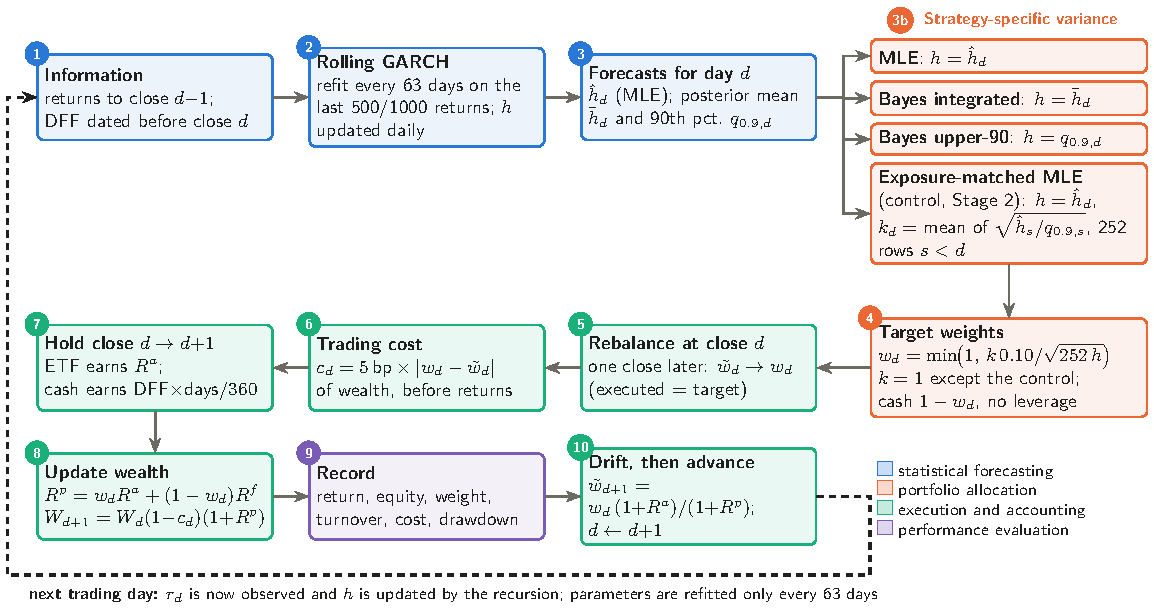
\includegraphics[width=\textwidth]{portfolio_flowchart.pdf}
\caption{Portfolio construction and simulation for trading day $d$. Blue: statistical forecasting; orange: portfolio
allocation; green: execution and accounting; purple: performance evaluation. The dashed loop returns to the
information step on the next trading day; parameters are refitted only on the 63-day schedule.}\label{fig:flow}
\end{figure}

\paragraph{Timing.} Forecast row $d$ uses returns up to the close of day $d-1$. Its weight is executed at the
\emph{close of day $d$}, one close later, and earns the close-to-close return from $d$ to $d+1$. This one-close delay
means that the price at which a trade is executed is never the price that produced the signal, and no forecast uses
a return that has not been observed.

\paragraph{Accounting.} Let $R^a_{d+1}=e^{r_{d+1}}-1$ be the ETF's simple return and $R^f_{d+1}$ the cash return over
the holding period. Wealth starts at $W_0=1$, entirely in cash. Each trading day:
\begin{align}
\tilde w_d&=\frac{w_{d-1}(1+R^a_d)}{1+R^p_d}\quad(\tilde w=0\text{ before the first trade}) &&\text{pre-trade (drifted) weight}\\
c_d&=0.0005\,\bigl|w_d-\tilde w_d\bigr| &&\text{cost fraction of wealth, 5 bp one-way}\\
R^p_{d+1}&=w_d\,R^a_{d+1}+(1-w_d)\,R^f_{d+1} &&\text{gross portfolio return}\\
W_{d+1}&=W_d\,(1-c_d)\,(1+R^p_{d+1}) &&\text{net wealth}
\end{align}
Three weights must be distinguished. The \emph{target} weight $w_d$ comes from the rule. The \emph{executed} weight
equals the target, because the portfolio is fully rebalanced every day; costs reduce wealth, not the weight. The
\emph{post-return} weight $\tilde w_{d+1}$ is the target after one day of drift: it rises when the ETF outperforms
cash. Drift is therefore distinct from deliberate rebalancing, and turnover $|w_d-\tilde w_d|$ measures only the trade
needed to undo it and move to the new target. Trading costs are charged on that turnover and are separate from market
returns. Cash earns the DFF rate dated strictly before the decision date, accrued as rate $\times$ calendar days$/360$ over
the holding period, so weekends and holidays accrue interest.

\paragraph{Performance metrics and why accuracy is not enough.} Each strategy is evaluated by the Sharpe ratio, the mean daily return in excess of the cash return divided by the
standard deviation of that excess return, multiplied by $\sqrt{252}$, the maximum drawdown (largest peak-to-trough loss of
wealth), the annualised return and volatility, the average ETF weight (risky exposure), average daily turnover and the
implied costs. A more accurate variance forecast need not improve these numbers: the weight responds to the
\emph{level} of the forecast, small forecast differences produce small weight differences, and simply holding less
risk changes volatility and drawdown on its own. Paired differences between strategies are assessed with a circular
block bootstrap \cite{politis1992} (20-day blocks, 2{,}000 replications), which preserves the dependence in daily returns.

% =====================================================================================================
\section{H3: portfolio evaluation in two stages}\label{sec:h3control}
The evaluation proceeds in two stages. Stage 1 compares the two rules of interest directly. Its result raises a
question that Stage 2 answers with a control experiment.

\subsection{Stage 1: Bayesian upper-90 versus standard MLE}\label{sec:stage1}
Table~\ref{tab:stage1} compares standard Gaussian GARCH MLE targeting with Bayesian upper-90 targeting in the primary
period, using means over the eight single-ETF asset--window configurations.

\begin{table}[h]\centering\small
\resizebox{.9\textwidth}{!}{\begin{tabular}{lrrrrr}\toprule
2017--22, mean of 8 single-ETF configurations & Exposure & Return & Volatility & Sharpe & Max DD\\\midrule
Standard MLE & 73.1\% & 6.25\% & 10.37\% & 0.518 & $-19.55\%$ \\
Bayesian upper-90 & 69.6\% & 6.06\% & 9.81\% & 0.520 & $-18.74\%$ \\
\midrule
Difference (upper-90 $-$ MLE) & $-3.6$ pp & $-0.19$ pp & $-0.55$ pp & $+0.002$ & $+0.82$ pp \\
Configurations whose 95\% CI excludes 0 & & & & 0 of 8 & 8 of 8 \\
\bottomrule\end{tabular}
}
\caption{Stage 1, 2017--22: standard MLE versus Bayesian upper-90, means over the 8 single-ETF configurations, 5 bp
costs. The last row counts configurations whose paired 95\% circular block-bootstrap interval for the difference
excludes zero.}\label{tab:stage1}
\end{table}

\paragraph{Observations.} Upper-90 has lower realised volatility (9.81\% versus 10.37\%) and a shallower maximum
drawdown, by 0.82 percentage points on average; its drawdown is smaller in all 8 configurations, and every paired
interval for the drawdown difference excludes zero. But it also holds 3.6 points less ETF and earns 0.19 points less
per year. Its Sharpe ratio is nearly unchanged ($+0.002$ on average): none of the 8 configuration intervals excludes
zero, and for the equal-weight four-ETF sleeve the differences are $+0.011$ $[-0.021,\,0.042]$ ($W=500$) and $+0.000$
$[-0.025,\,0.026]$ ($W=1000$). The 2023--26 period shows the same pattern (4.1 points less exposure, drawdown smaller in
8 of 8).

\paragraph{Interpretation.} Upper-90 takes less risk at almost the same risk-adjusted return, which is the pattern a
lower volatility target would also produce: scaling all weights by a constant shrinks volatility and drawdown roughly
proportionally and leaves the Sharpe ratio almost unchanged. The drawdown gain is real, but Table~\ref{tab:stage1}
cannot say what causes it.

\keybox{\textbf{Question raised by Stage 1.} Does Bayesian uncertainty improve allocation \emph{timing}, or is the lower
drawdown simply a consequence of \emph{holding less risk}?}

\subsection{Stage 2: the exposure-matched MLE control}\label{sec:stage2}
\paragraph{Objective.} Build a strategy that holds the same average risk as upper-90 but uses no posterior
information. If upper-90's advantage is only lower exposure (explanation A), the two should perform alike; if the
posterior tells the strategy \emph{when} to reduce risk (explanation B), upper-90 should still win.

\paragraph{Allocation rule and calibration.} The control keeps the MLE variance forecast unchanged and scales only the
volatility target:
\begin{equation}\label{eq:control}
\begin{gathered}
w_d^{\text{MLE,control}}=\min\Bigl(1,\ \frac{k_d\cdot0.10}{\sqrt{252\,\hat h_d}}\Bigr),\\
k_d=\frac{1}{d-\max(0,d-252)}\sum_{s=\max(0,d-252)}^{d-1}\sqrt{\frac{\hat h_s}{q_{0.9,s}}}\quad(d\ge1),\qquad k_0=\sqrt{\hat h_0/q_{0.9,0}}.
\end{gathered}
\end{equation}
The scaling factor $k_d$ is the trailing mean, over up to 252 earlier forecast rows of the evaluation segment, of the
ratio between the MLE and upper-90 volatility forecasts, which is exactly the ratio of their uncapped weights
(\texttt{bgarch.portfolio.exposure\_matched\_weights}). It changes the \emph{effective volatility target}, $0.10\,k_d$,
not the GARCH parameters or the variance forecast. The implementation:
\begin{itemize}
\item uses only information available before day $d$: the forecasts of rows $s<d$, each itself formed from earlier
returns (the first row uses its own forecast ratio, which is known at decision time); no realised return enters $k_d$
directly;
\item matches upper-90's \emph{average haircut}, not its realised exposure; because weights are capped at one, average
exposure is matched only approximately;
\item does \emph{not} incorporate parameter uncertainty into the MLE forecast: $k_d$ changes only slowly, so the control
carries none of the day-to-day posterior information;
\item keeps the investment universe, execution timing, costs and cash accounting identical.
\end{itemize}
The match is close: the control's mean exposure differs from upper-90's by $+0.1$ percentage points in 2017--22 (range
$-0.06$ to $+0.41$ across configurations) and $-0.3$ points in 2023--26 (range $-1.32$ to $+0.10$). Equal average
exposure does not guarantee identical daily exposure, volatility or tail risk. Figure~\ref{fig:w} shows why the
comparison is informative: the upper-90 weights are close to a constant haircut of the MLE weights, and the control
tracks them.

\begin{figure}[h]\centering
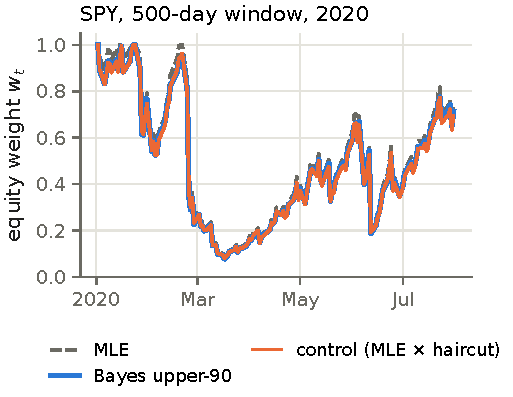
\includegraphics[width=.55\textwidth]{weights_spy2020.pdf}
\caption{SPY, 500-day window, January--July 2020: ETF weights of standard MLE, Bayesian upper-90 and the exposure-matched
MLE control (from the saved forecasts). The upper-90 weights are nearly a constant haircut of the MLE weights, and the
control tracks them closely.}\label{fig:w}
\end{figure}

\subsection{Stage 2 results: upper-90 versus exposure-matched MLE}\label{sec:stage2res}
\begin{table}[h]\centering\small
\resizebox{.9\textwidth}{!}{\begin{tabular}{lrrrrr}\toprule
2017--22, mean of 8 single-ETF configurations & Exposure & Return & Volatility & Sharpe & Max DD\\\midrule
Exposure-matched MLE & 69.4\% & 6.01\% & 9.85\% & 0.516 & $-18.66\%$ \\
Bayesian upper-90 & 69.6\% & 6.06\% & 9.81\% & 0.520 & $-18.74\%$ \\
\midrule
Difference (upper-90 $-$ matched MLE) & $+0.1$ pp & $+0.04$ pp & $-0.03$ pp & $+0.003$ & $-0.07$ pp \\
Configurations whose 95\% CI excludes 0 & & & & 0 of 8 & 0 of 8 \\
\bottomrule\end{tabular}
}
\caption{Stage 2, 2017--22: exposure-matched MLE versus Bayesian upper-90, means over the 8 single-ETF configurations,
5 bp costs. The last row counts configurations whose paired 95\% block-bootstrap interval excludes zero.}\label{tab:stage2}
\end{table}

\paragraph{Observations.} Once average exposure is matched ($+0.1$ points), realised volatility ($9.81\%$ versus
$9.85\%$), maximum drawdown ($-18.74\%$ versus $-18.66\%$) and the Sharpe ratio ($0.520$ versus $0.516$) are very similar
(Table~\ref{tab:stage2}). Upper-90's drawdown is smaller in only 2 of 8 configurations, and no configuration interval
excludes zero for either the Sharpe or the drawdown difference. For the four-ETF sleeve the Sharpe differences are
$+0.009$ $[-0.016,\,0.036]$ and $+0.005$ $[-0.016,\,0.027]$, and the drawdown differences $-0.01$ $[-0.22,\,0.43]$ and
$-0.03$ $[-0.20,\,0.45]$ points, whereas against MLE the sleeve drawdown intervals excluded zero ($+0.76$
$[0.22,\,1.21]$ and $+0.55$ $[0.11,\,1.01]$). Every 95\% interval for the sleeve Sharpe difference between upper-90 and
MLE, the control, or the classical Laplace upper-90 rule contains zero, in both periods (Table~\ref{tab:paired},
Figure~\ref{fig:sh}). Figure~\ref{fig:exp} shows the same thing configuration by configuration, and
Table~\ref{tab:exp} for both periods: against the control, the drawdown difference is $-0.07$ and $+0.09$ points and the
mean Sharpe difference $+0.003$ and $-0.001$.

\paragraph{Interpretation.} The Stage 1 drawdown advantage is reproduced by a strategy that simply holds the same
average risk without any posterior information, so the evidence supports explanation A. Point estimates of the Sharpe
difference are small and of either sign, and their intervals are a few hundredths wide, so no statistically reliable
incremental benefit is established; rounded point estimates should not be read as either a gain or a loss. For the
sleeve as a whole (Table~\ref{tab:alloc}), the Gaussian-GARCH rules (MLE, MAP, Bayesian, Laplace and the controls) have
Sharpe ratios within about 0.02 of one another in each period; including Student-$t$ GARCH, the spread reaches 0.047 in
2017--22. Costs of 0, 5 and 20 bp do not reverse any conclusion (Appendix~\ref{app:robust}).

\begin{figure}[h]\centering
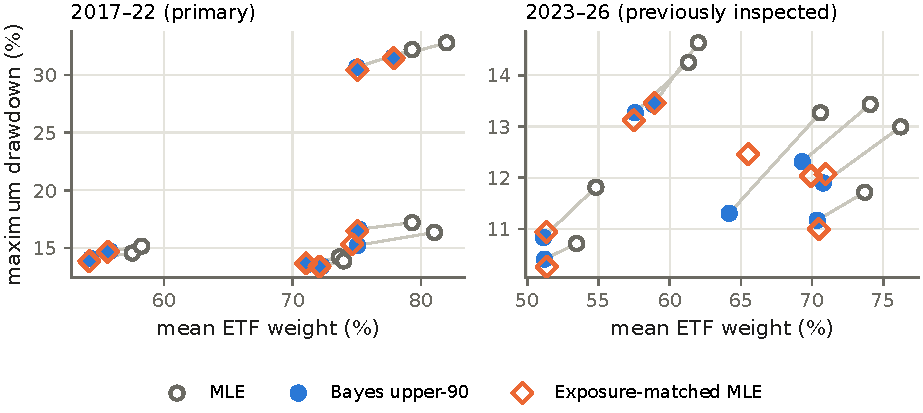
\includegraphics[width=.85\textwidth]{exposure_control.pdf}
\caption{Mean ETF weight against maximum drawdown for each asset--window configuration. Grey lines join MLE to Bayes
upper-90 (Stage 1); the exposure-matched MLE control (diamonds, Stage 2) lands on top of upper-90.}\label{fig:exp}
\end{figure}

\begin{table}[h]\centering\small
\begin{tabular}{lrrrr}\toprule
Period & $\Delta$exposure (pp) & $\Delta$MaxDD vs MLE (pp) & $\Delta$MaxDD vs control (pp) & $\Delta$Sharpe vs control\\\midrule
2017--22 & -3.6 & +0.82 (8/8) & -0.07 (2/8) & +0.0034 (6/8) \\
2023--26 & -4.1 & +1.02 (8/8) & +0.09 (4/8) & -0.0011 (2/8) \\
\bottomrule\end{tabular}

\caption{Upper-90 minus comparators in both periods, averaged over the 8 asset--window configurations. Counts give the
number of configurations with a positive difference. pp = percentage points.}\label{tab:exp}
\end{table}

\begin{table}[h]\centering\footnotesize
\resizebox{\textwidth}{!}{\begin{tabular}{lrrrrrrrr}\toprule
 & \multicolumn{4}{c}{2017--22} & \multicolumn{4}{c}{2023--26}\\\cmidrule(lr){2-5}\cmidrule(lr){6-9}
 & \multicolumn{2}{c}{Sharpe} & \multicolumn{2}{c}{Max DD (\%)} & \multicolumn{2}{c}{Sharpe} & \multicolumn{2}{c}{Max DD (\%)}\\
Strategy & 500 & 1000 & 500 & 1000 & 500 & 1000 & 500 & 1000\\\midrule
Buy and hold & 0.695 & 0.695 & -25.2 & -25.2 & 1.086 & 1.086 & -10.3 & -10.3 \\
Static weight (pre-period calibrated) & 0.677 & 0.677 & -18.3 & -18.3 & 1.019 & 1.019 & -5.8 & -5.8 \\
EWMA & 0.884 & 0.884 & -13.2 & -13.2 & 0.926 & 0.926 & -7.6 & -7.6 \\
Student-$t$ GARCH (MLE) & 0.903 & 0.864 & -13.9 & -14.3 & 0.929 & 0.892 & -6.9 & -6.9 \\
Gaussian GARCH, MLE & 0.864 & 0.849 & -14.1 & -14.5 & 0.917 & 0.887 & -6.8 & -6.8 \\
Bayes, integrated variance & 0.870 & 0.851 & -14.2 & -14.6 & 0.924 & 0.895 & -6.6 & -6.8 \\
Bayes, upper-90\% variance & 0.875 & 0.849 & -13.3 & -14.0 & 0.925 & 0.887 & -6.1 & -6.5 \\
MLE $\times$ real-time haircut (control) & 0.866 & 0.844 & -13.3 & -14.0 & 0.918 & 0.895 & -6.5 & -6.5 \\
Laplace (classical) upper-90\% & 0.856 & 0.849 & -13.3 & -14.0 & 0.926 & 0.884 & -5.8 & -6.5 \\
\bottomrule\end{tabular}
}
\caption{Equal-weight four-ETF sleeve, 5 bp costs, 10\% volatility target. ``500/1000'' are estimation windows (rows
without a window use the same series).}\label{tab:alloc}
\end{table}

\begin{table}[h]\centering\footnotesize
\resizebox{\textwidth}{!}{\begin{tabular}{lcccc}\toprule
 & \multicolumn{2}{c}{2017--22} & \multicolumn{2}{c}{2023--26}\\\cmidrule(lr){2-3}\cmidrule(lr){4-5}
$\Delta$Sharpe [95\% block-bootstrap CI] & $W{=}500$ & $W{=}1000$ & $W{=}500$ & $W{=}1000$\\\midrule
Upper-90 $-$ MLE & +0.011 [-0.021, +0.042] & +0.000 [-0.025, +0.026] & +0.009 [-0.027, +0.042] & +0.000 [-0.027, +0.026] \\
Upper-90 $-$ MLE$\times$haircut (control) & +0.009 [-0.016, +0.036] & +0.005 [-0.016, +0.027] & +0.008 [-0.026, +0.043] & -0.008 [-0.031, +0.017] \\
Upper-90 $-$ Laplace upper-90 & +0.019 [-0.001, +0.042] & +0.000 [-0.010, +0.013] & -0.000 [-0.033, +0.029] & +0.003 [-0.006, +0.013] \\
Integrated $-$ MLE & +0.005 [-0.010, +0.021] & +0.002 [-0.012, +0.018] & +0.007 [-0.019, +0.032] & +0.008 [-0.005, +0.021] \\
\bottomrule\end{tabular}
}
\caption{Paired Sharpe-ratio differences for the four-ETF sleeve with circular block-bootstrap 95\% intervals.}\label{tab:paired}
\end{table}

\begin{figure}[h]\centering
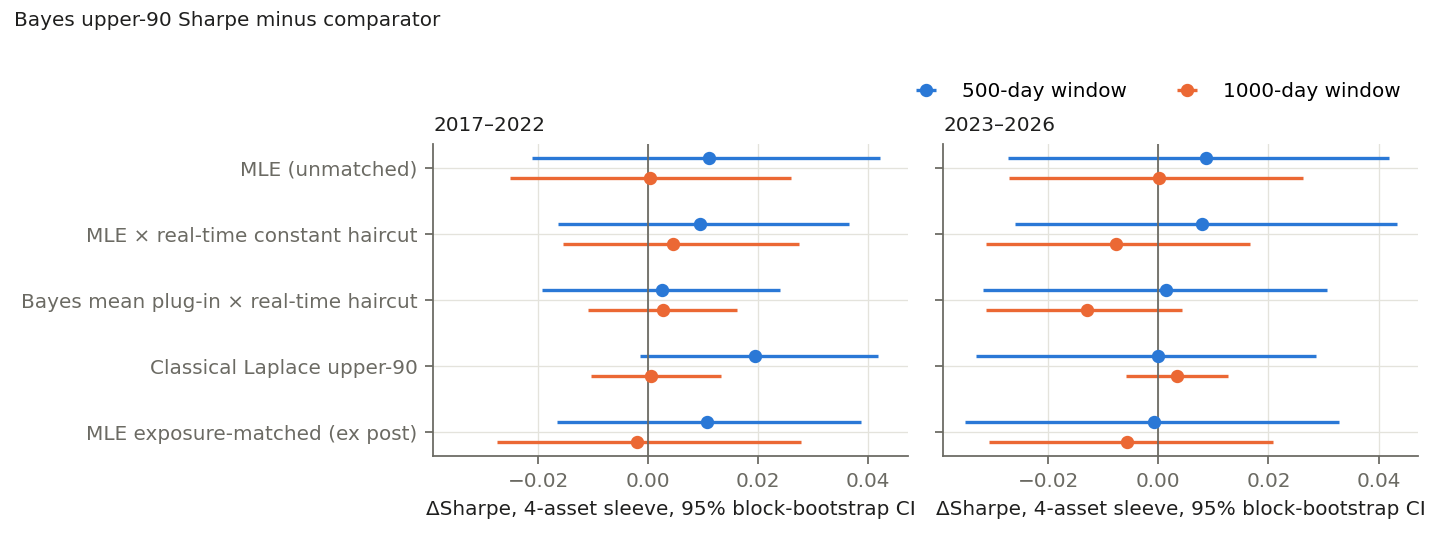
\includegraphics[width=.9\textwidth]{fig2_sharpe_differences.png}
\caption{Upper-90 Sharpe ratio minus comparators (four-ETF sleeve), with 95\% block-bootstrap intervals.}\label{fig:sh}
\end{figure}

\paragraph{Conclusion for H3.} The conservative Bayesian rule reduces exposure and drawdowns relative to MLE, but
exposure matching removes the apparent advantage, and no statistically reliable incremental improvement in portfolio
performance is established. \textbf{H3 is not supported.}
\keybox{\textbf{Finding 2.} The observed drawdown reduction is largely consistent with reduced risky exposure rather
than demonstrably superior risk timing from Bayesian parameter uncertainty. Better-looking portfolio performance must
be examined against appropriately controlled alternatives.}
\noindent This does not rule out every possible benefit of Bayesian inference for allocation: other decision rules,
objectives or models might use the posterior differently. Exposure matching is also not a perfect control for all
differences in portfolio risk.

% =====================================================================================================
\section{Limitations and future research}\label{sec:limits}
\paragraph{Limitations of the tested design.}
\begin{itemize}
\item \textbf{Innovation misspecification.} Only symmetric Gaussian GARCH(1,1) receives a Bayesian treatment. Equity
residuals are also negatively skewed, which no symmetric model captures (Appendix~\ref{app:adequacy}).
\item \textbf{Estimation design.} Rolling windows are finite (500 or 1000 days) and parameters are refitted quarterly
rather than daily. The MLE persistence bound binds in 30 of 320 refits.
\item \textbf{Monte Carlo uncertainty.} Bayesian results reproduce only to Monte Carlo precision across platforms;
across three seeds a configuration's upper-90 Sharpe ratio varies by up to 0.010.
\item \textbf{Regimes and dependence.} Four ETFs, six plus four years, regime shifts (for example in bond volatility
in 2020--22) and serially dependent score and return differences limit power: Sharpe differences below about 0.05
cannot be resolved.
\item \textbf{Execution assumptions.} Yahoo adjusted closes, close-to-close execution one close after the signal, a
proportional 5 bp cost and DFF as the cash rate are approximations shared by all methods.
\item \textbf{Exposure matching} equalises average exposure only approximately and does not equalise daily risk.
\end{itemize}

\paragraph{Future research (not tested here).}
\begin{itemize}
\item Bayesian Student-$t$ GARCH, and skewed-$t$ or other flexible innovation distributions.
\item More informative or hierarchical priors shared across assets.
\item Alternative risk objectives and utility functions; allocation based on posterior expected shortfall or tail risk.
\item Other uncertainty-aware decision rules, evaluated against matched controls from the outset.
\end{itemize}

% =====================================================================================================
\section{Summary and scientific conclusions}\label{sec:summary}
\paragraph{H1 --- conditional variance.} Bayesian posterior integration produces small numerical QLIKE improvements,
but they are not statistically reliable at the conventional 5\% level in the primary evaluation.

\paragraph{H2 --- predictive distributions.} Bayesian parameter integration modestly improves the predictive return
density (0.002--0.005 nats per day, significant in every cell), and a classical Laplace approximation achieves 43--89\%
of that gain. Student-$t$ GARCH estimated by MLE produces substantially larger improvements, five to six times as large
in 2017--2022, which indicates that innovation-distribution specification matters more than Gaussian GARCH parameter
uncertainty in the tested setting.

\paragraph{H3 --- portfolio allocation.} Conservative Bayesian allocation tends to reduce risky exposure and
drawdowns. After comparison with exposure-matched MLE, the project does not establish a statistically reliable
incremental investment benefit.

\paragraph{Two central takeaways.}
\begin{enumerate}
\item Better modelling of heavy-tailed innovations can matter more for predictive density accuracy than integrating
parameter uncertainty under a misspecified Gaussian model.
\item Better-looking portfolio performance must be examined against appropriately controlled alternatives. Lower
drawdown is not necessarily evidence of better forecasting or investment timing when average exposure also decreases.
\end{enumerate}

\paragraph{Overall conclusion.} Better probabilistic forecasts do not automatically translate into economically
better investment decisions. Model specification, uncertainty quantification and fair, risk-controlled experiments
are all essential to evaluating practical value. These conclusions hold across two evaluation periods, two
estimation windows, three Monte Carlo seeds and two priors.

{\small
\bibliographystyle{unsrtnat}
\bibliography{references}}

\appendix
% =====================================================================================================
\section{Model adequacy: out-of-sample diagnostics}\label{app:adequacy}
This appendix checks which features of the returns the fitted models reproduce, supporting the H2 interpretation. It
uses the saved one-step-ahead forecasts for 2017--2022 with the 500-day window ($n=1{,}510$ per ETF); nothing is
refitted. Every forecast $h_d$ uses parameters fitted before day $d$, so $z_d=r_d/\sqrt{h_d}$ and the probability
integral transform $u_d=F_d(r_d)$ are genuine out-of-sample quantities rather than in-sample residuals. For the
Bayesian mixture, $u_d=M^{-1}\sum_m\Phi(r_d/\sqrt{h_d^{(m)}})$ uses the full predictive CDF \cite{diebold1998}. Under
correct calibration $\Phi^{-1}(u_d)\sim N(0,1)$ \cite{berkowitz2001}. Ljung--Box \cite{ljungbox1978} tests on $z_d^2$
(McLeod--Li \cite{mcleodli1983}) detect remaining volatility clustering. Their nominal $p$-values ignore estimation
error and serial dependence and are therefore approximate.

\begin{table}[h]\centering
\resizebox{\textwidth}{!}{\begin{tabular}{llllrrrrrr}\toprule
 & ACF$_1(r^2)$ & Model & ACF$_1(z^2)$ & LB$_{10}(z^2)$ $p$ & skew $z$ & ex.\ kurt $\Phi^{-1}$(PIT) & lower 1\% & upper 1\% & KS(PIT) $p$\\\midrule
SPY & 0.46 & Gaussian MLE & +0.01 & .076 & -0.85 & 2.91 & 2.5 & 0.9 & <.001 \\
 &  & Bayes mixture & +0.01 & .092 & -0.85 & 2.70 & 2.5 & 0.9 & <.001 \\
 &  & Student-$t$ & +0.02 & .365 & -0.88 & 0.01 & 1.7 & 0.3 & <.001 \\
\midrule
QQQ & 0.43 & Gaussian MLE & -0.02 & .040 & -0.67 & 1.95 & 2.5 & 0.7 & <.001 \\
 &  & Bayes mixture & -0.03 & .039 & -0.66 & 1.81 & 2.5 & 0.7 & <.001 \\
 &  & Student-$t$ & -0.02 & .330 & -0.67 & 0.03 & 1.8 & 0.5 & <.001 \\
\midrule
TLT & 0.51 & Gaussian MLE & +0.11 & <.001 & +0.04 & 0.97 & 1.7 & 1.5 & .567 \\
 &  & Bayes mixture & +0.06 & <.001 & +0.03 & 0.54 & 1.4 & 1.7 & .579 \\
 &  & Student-$t$ & +0.11 & <.001 & +0.05 & 0.35 & 1.5 & 1.5 & .303 \\
\midrule
GLD & 0.12 & Gaussian MLE & -0.01 & <.001 & -0.26 & 1.90 & 1.8 & 1.9 & <.001 \\
 &  & Bayes mixture & -0.01 & <.001 & -0.26 & 1.83 & 1.8 & 1.5 & <.001 \\
 &  & Student-$t$ & -0.01 & <.001 & -0.26 & 0.08 & 1.1 & 1.1 & .002 \\
\bottomrule\end{tabular}
}
\caption{Out-of-sample diagnostics, 2017--22, 500-day window. ACF$_1$: lag-1 autocorrelation. ``lower/upper 1\%'' are
the percentages of days with $u_d<0.01$ / $u_d>0.99$ (nominal 1\%; about $\pm0.5$ pp is two binomial standard
errors).}\label{tab:adequacy}
\end{table}

\begin{figure}[h]\centering
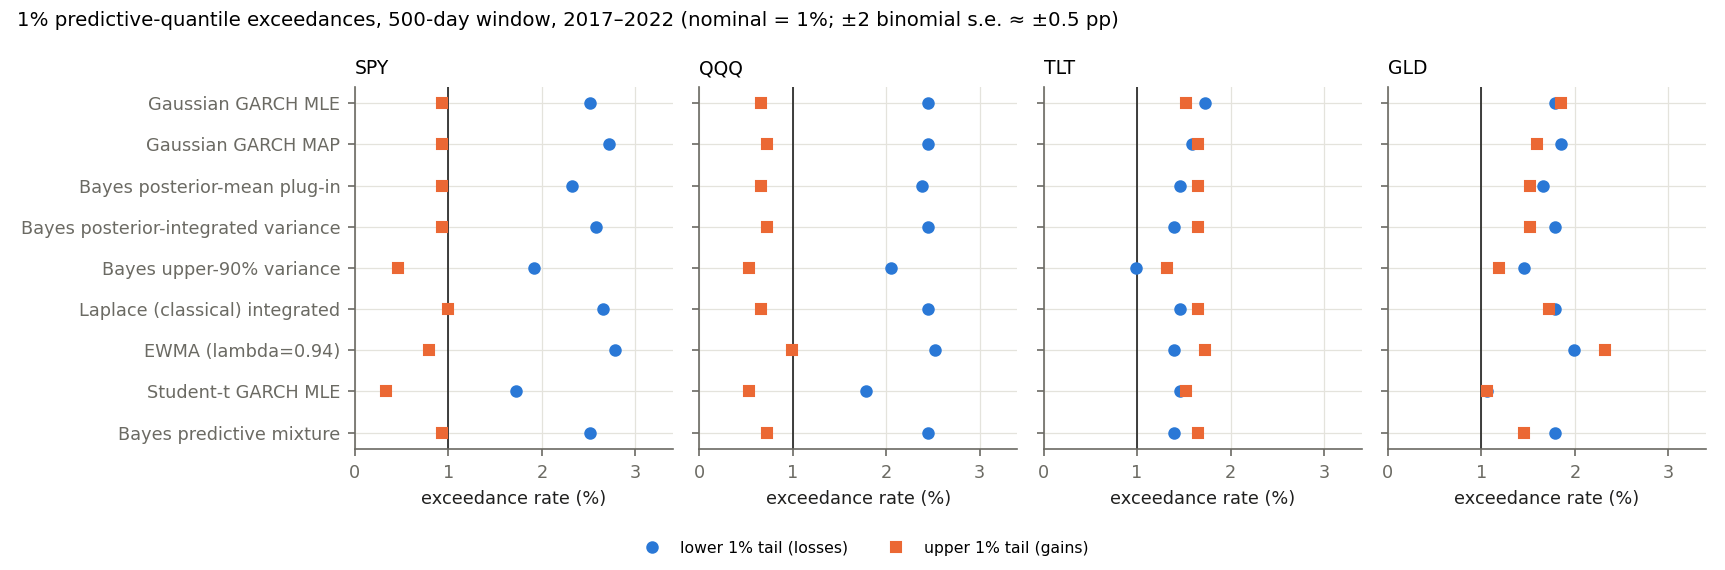
\includegraphics[width=\textwidth]{adequacy_exceedance_summary.png}
\caption{1\% predictive-quantile exceedances for all nine forecast distributions.}\label{fig:exceed}
\end{figure}

\noindent\textbf{Conclusions supported by the diagnostics.}
\begin{itemize}
\item \textbf{Clustering is mostly captured.} Squared returns have lag-1 autocorrelation 0.43--0.51 for SPY, QQQ and TLT.
After standardising by the GARCH forecast it is about 0 for SPY and QQQ. TLT retains about 0.1 up to lag 8
($p<0.001$), a sign of bond-volatility regime shifts in 2020--22 that a quarterly-refitted GARCH(1,1) absorbs only partly.
\item \textbf{Gaussian tails are too thin.} The excess kurtosis of $z$ is 1.9--2.9 for SPY, QQQ and GLD. Over 2017--26, $|z|>3$
occurs on 23--33 of 2{,}474 days per ETF against 6.7 expected. Lower-tail 1\% exceedances reach 2.5\% for SPY
and QQQ. The Bayesian mixture changes this hardly at all: the excess kurtosis of its normal scores falls only from 2.9 to 2.7 for SPY.
\item \textbf{Student-$t$ fixes symmetric fat tails but not asymmetry.} Its normal scores have excess kurtosis near 0,
and GLD's tails become well calibrated. Equity residuals, however, are negatively skewed ($-0.67$ to $-0.85$).
Every symmetric model has too many lower-tail and too few upper-tail exceedances (SPY Student-$t$: 1.7\% and
0.3\%), and the PIT is rejected for all equity models.
\item \textbf{Hard cases.} The most 1\% breaches occur when \emph{predicted} volatility is low (SPY and QQQ: about 3\%
in the calm tercile), and in 2018 and 2020, when shocks arrived out of calm markets. In stress periods every
GARCH variant reacts on the next day and decays with a half-life of 9--16 trading days. EWMA reacts more slowly
and stays elevated two to three times longer.
\end{itemize}
These results explain the main findings. Parameter uncertainty is a second-order source of misspecification;
innovation shape and asymmetry are first-order. Fitting asymmetric models is outside the scope of this study.

% =====================================================================================================
\section{Secondary robustness results}\label{app:robust}
\paragraph{MLE persistence bound.} In 30 of the 320 refits the Gaussian MLE stops on the bound $p\le0.99909$.
Relaxing the bound changes the log-likelihood by at most 1.15 but moves next-day variance by a median of 5\%. We keep
the original bound to preserve the estimator's definition and treat it as a limitation.

\paragraph{Monte Carlo variability.} Rerunning the original project with the \emph{same} seed on a different machine
changed Bayesian variance quantiles by 0.5--1.7\%, and two fits that had passed the strict diagnostics failed them
marginally ($\hat R=1.010$--$1.011$). Across three seeds, a configuration's upper-90 Sharpe ratio varies by up to 0.010.
Classical quantities reproduce to $10^{-12}$.

\paragraph{Does posterior uncertainty predict when forecasts fail?} The ``uncertainty premium'' $q_{0.9}/\bar h-1$ is
almost a deterministic function of the variance level (correlation $>0.99$). In HAC regressions of absolute forecast
errors and large-shock indicators on the premium, 4 of 32 coefficients are significant at 5\%, close to what chance
would produce (1.6 expected), with mixed signs.

\paragraph{Other robustness.} A broad prior ($\logit p\sim N(0,3^2)$) gives the same conclusions, although it causes
more convergence failures, including a bimodal posterior for TLT. The forecast comparisons are unchanged when days from
refits that fail diagnostics are excluded. Costs of 0, 5 and 20 bp do not reverse any conclusion. An exploratory search
for uncertainty-aware strategies was pre-registered with a validation gate. None of the three candidates passed, so
the final holdout was never used (see the research report).

% =====================================================================================================
\section{Data provenance}\label{app:data}
\begin{itemize}
\item \textbf{ETF prices:} Yahoo Finance daily closes for SPY, QQQ, TLT and GLD, downloaded with \texttt{yfinance} using \texttt{auto\_adjust=True} (split- and dividend-adjusted closes), 2013-01-02 to 2026-11-04, stored locally in \texttt{data/*\_adjusted.csv}. Unadjusted closes were not stored. Yahoo's terms restrict redistribution, so these files are not included in the public repository.
\item \textbf{Cash rate:} Board of Governors of the Federal Reserve System, Effective Federal Funds Rate (DFF), retrieved from FRED, Federal Reserve Bank of St.~Louis; stored as \texttt{data/DFF.csv}, last observation 2026-11-03.
\end{itemize}

% =====================================================================================================
\section{Reproduction}\label{app:repro}
From the repository root, after \texttt{pip install -e .} (the saved rolling artifacts and the market data are not distributed; see the repository README):
\begin{itemize}
\item \texttt{pytest} --- 54 tests covering the likelihood, forecast timing, portfolio accounting, reproduction of saved results and the adequacy diagnostics;
\item \texttt{python -m bgarch.reproduce quick} --- verifies 48 artifact checksums and regenerates every table and figure in about 25\,s;
\item \texttt{python -m bgarch.reproduce full --out NEW\_DIR} --- reruns all 320 refits, 16 jobs, in about 70\,s on 7 cores of an Apple M3;
\item \texttt{python scripts/make\_report\_tables.py} --- writes the tables of this report from the quick-mode output;
\item \texttt{python scripts/make\_narrative\_figures.py --diagrams} --- the narrative figures and the two diagrams (Figures~\ref{fig:design}, \ref{fig:qlike}, \ref{fig:dens}, \ref{fig:flow}, \ref{fig:exp}).
\end{itemize}
On the development machine, full mode reproduced every reported table entry exactly. On other platforms, Bayesian
columns may differ at Monte Carlo precision. The executed notebook \texttt{notebooks/walkthrough.ipynb} rederives each step and
runs numerical checks against the saved results; \texttt{notebooks/quick\_walkthrough.ipynb} is a concise, independent version.
\texttt{python -m bgarch.adequacy} regenerates Appendix~\ref{app:adequacy} (about 8\,s).

\section{AI-assistance disclosure}
The independent audit, the 2017--2022 replication, the analysis code, the course package, this report and the
accompanying notebooks were produced with substantial assistance from an AI system (Claude, by Anthropic, used
through Claude Code) working in the author's project directory under the author's direction. The AI wrote and ran
code, executed the experiments and drafted text. All quantitative statements were checked programmatically against
saved artifacts by the automated tests and notebook checks described above. The author is responsible for
verifying, understanding and presenting the work.
\end{document}
